
\documentclass{article}
\usepackage{fullpage}
\usepackage{color}
\usepackage[normalem]{ulem}
\usepackage{hyperref}
\usepackage{enumitem}
\usepackage{graphicx}
\hypersetup{colorlinks}
\hyphenpenalty=100000
\begin{document}
\setlength{\voffset}{3.5in}
\title{Architecture}
\author{\Large Android Based Situational Awareness: Moving Map\\
Tom Atnip, Susi Cisneros, Sam Kim, and Seth Troisi}
\date{\today}
\maketitle
\clearpage
\setlength{\voffset}{0pt}
\tableofcontents
\clearpage
~\\
\begin{Large}\textbf{Changes}\end{Large}\\
~\\
\begin{tabular}{ | p{1.5in} | p{4.5in} | }
\hline
\textbf{Date} & \textbf{Description}\\
\hline
\hline
October 4, 2012 & Document created\\
\hline
October 15, 2012 & Added Introduction\\
\hline
\end{tabular}
\clearpage

\section{Introduction}
This document provides a high-level overview of the components of the system.

\section{System Diagrams}
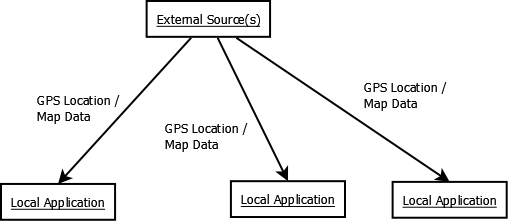
\includegraphics[keepaspectratio, width=5in]{HighLevelSystemView.png} \\
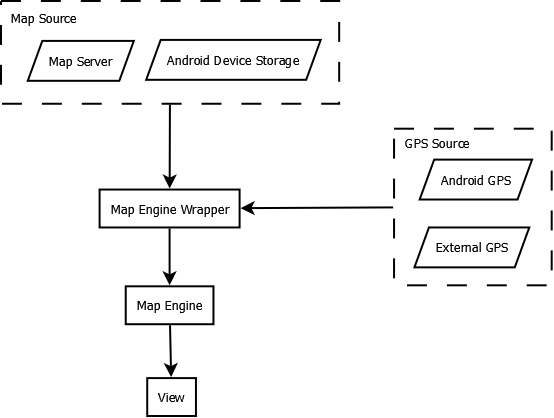
\includegraphics[keepaspectratio, width=5in]{NotDataFlowDiagram.png} \\
\section{Package Diagrams}
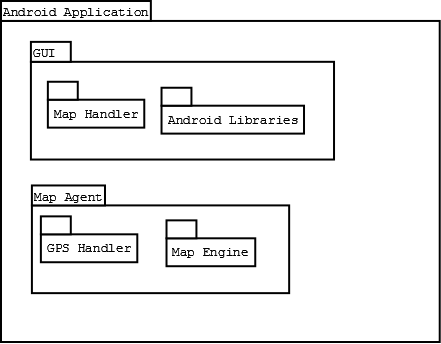
\includegraphics[keepaspectratio, width=5in]{ProjectUMLDiagram.png} \\
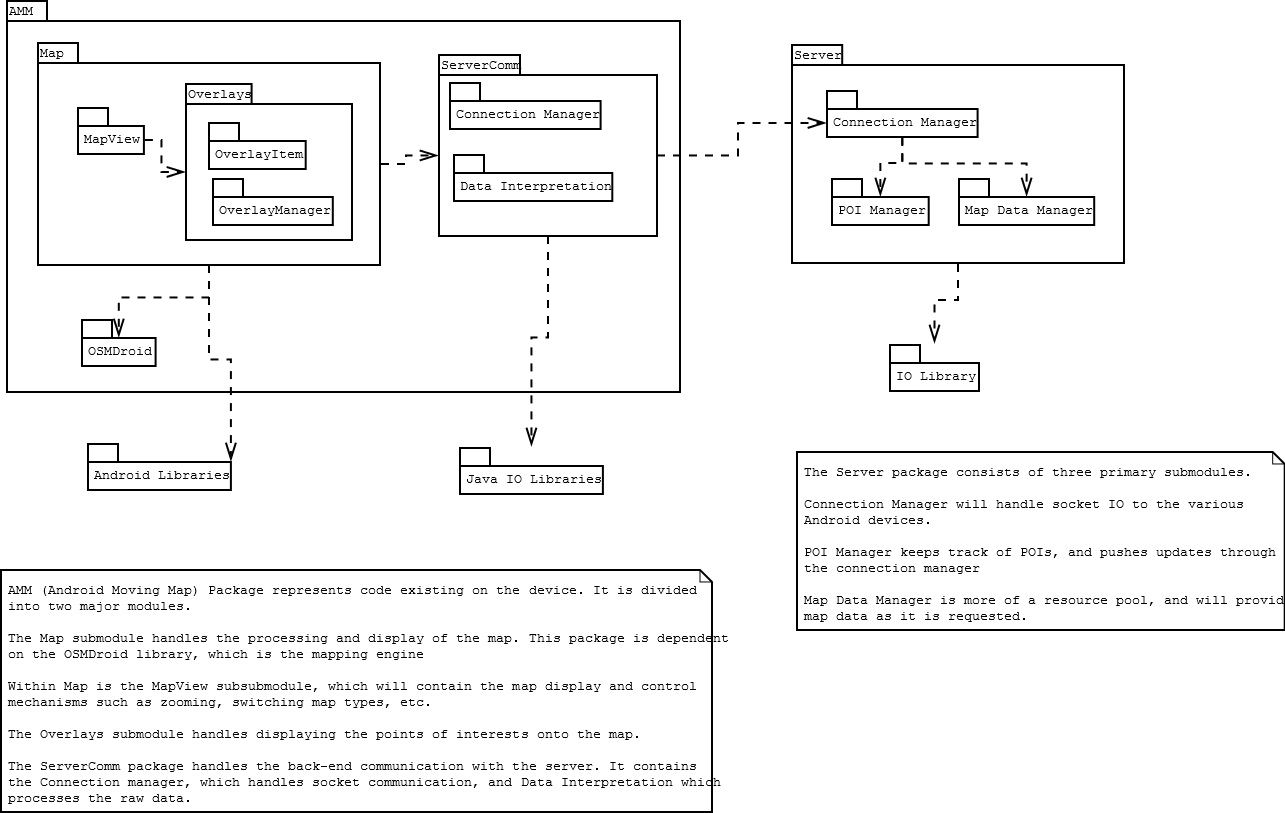
\includegraphics[keepaspectratio, width=7in]{package.png} \\
AMM:\\
AMM (Android Moving Map) Package represents code existing on the device.  It is divided into two major modules.  The Map submodule handles the processing and display of the map.  This package is dependent on the OSMDroid library, which is the mapping engine.
Within the Map is the MapView subsubmodule, which will contain the map display and control mechanisms such as zooming, switching map types, etc.  The Overlays submodule handles displaying the points of interests onto the map.  The ServerComm package handles the back-end communication with the server.  It contains the Connection manager, which handles socket communication, and data interpretation which processes the raw data.\\ \\
Server:\\
The Server package consists of three primary submodules.  Connection Manager will handle socket IO to the various Android devices.  POI Manager keeps track of POIs, and pushes updates through the connection manager.  Map Data Manager is more of a resource pool, and will provide map data as it is requested.

\end{document}